\documentclass[11pt,twoside]{article}
\usepackage[T1]{fontenc}
\usepackage[utf8]{inputenc}
\usepackage[english]{babel}
\usepackage{amsmath}
\usepackage{amscd}
\usepackage{amssymb}
\usepackage{multirow}
\usepackage{tabularx}
\usepackage{graphicx}
\usepackage{url}
\usepackage{fancyhdr}
\usepackage{MnSymbol,wasysym}
\usepackage{lastpage}
\usepackage[a4paper,margin=2.5cm,hmarginratio=1:1]{geometry}

\newtheorem{theorem}{Theorem}[section]
\newtheorem{proof}{Proofsketch}[section]

%%%%%%%%%%%%%%%%%%%%%%%%%%%%%%%%%%%%%%%%%%%%%%%%%%%%%%%%%%%%%%%%%%%%%%%%%%%
%%%%%%%%%%%%%% ENTER YOUR PERSONAL INFORMATION HERE %%%%%%%%%%%%%%%%%%%%%%%
%%%%%%%%%%%%%%%%%%%%%%%%%%%%%%%%%%%%%%%%%%%%%%%%%%%%%%%%%%%%%%%%%%%%%%%%%%%


% Your name, personal number, and email.
\newcommand{\firstname}{Bastian}
\newcommand{\lastnames}{Fredriksson}
\newcommand{\persnr}{9302164216}
\newcommand{\email}{bastianf@kth.se}


% Your two study pals. Leave empty as necessary.
\newcommand{\studypalX}{Fabian Ström}
\newcommand{\studypalXemail}{fabstr@kth.se}
\newcommand{\studypalY}{}
\newcommand{\studypalYemail}{}


%%%%%%%%%%%%%%%%%%%%%%%%%%%%%%%%%%%%%%%%%%%%%%%%%%%%%%%%%%%%%%%%%%%%%%%%%%%
%%%%%%%%%%%%% DO NOT TOUCH ANYTHING BELOW THIS LINE %%%%%%%%%%%%%%%%%%%%%%%
%%%%%%%%%%%%%%%%%%%%%%%%%%%%%%%%%%%%%%%%%%%%%%%%%%%%%%%%%%%%%%%%%%%%%%%%%%%

\newcounter{problem}
\renewcommand\theproblem{\arabic{problem}}
\newenvironment{problem}{%
  \bigbreak
  \refstepcounter{problem}\noindent
  \llap{\textbf{\theproblem}\quad}\ignorespaces
}{%
  \par\if@nadaten@solutions\relax\else\filbreak\fi
}
\newenvironment{problem*}{%
  \bigbreak
  \refstepcounter{problem}\noindent
  \llap{\textbf{\theproblem}\quad}\ignorespaces
}{%
  \par
}
\newcounter{subproblem}[problem]
\renewcommand{\thesubproblem}{\arabic{problem}\alph{subproblem}}
\newenvironment{subproblem}{%
  \refstepcounter{subproblem}%
  \list{}{}%
  \item\leavevmode
  \llap{\hbox to \leftmargini{\textbf{\thesubproblem}\hfil}}%
  \ignorespaces
}{%
  \endlist\if@nadaten@solutions\relax\else\filbreak\fi
}
\newenvironment{subproblem*}{%
  \refstepcounter{subproblem}%
  \list{}{}%
  \item\leavevmode
  \llap{\hbox to \leftmargini{\textbf{\thesubproblem}\hfil}}%
  \ignorespaces
}{%
  \endlist
}

\newcommand{\homeworknr}{4}
\newcommand{\studentname}{\firstname~\lastnames}
\newcommand{\homework}{Homework~\homeworknr}
\newcommand{\coursenumber}{DD2448}
\newcommand{\coursename}{\coursenumber~Foundations of cryptography}
\newcommand{\coursenick}{krypto15}

\lhead[\studentname]{\coursename}
\chead{}
\rhead[\coursename]{\studentname}
\lfoot[\thepage~(\pageref{LastPage})]{}
\cfoot{}
\rfoot[]{\thepage~(\pageref{LastPage})}

\fancypagestyle{firststyle}
{
   \fancyhf{}
   \fancyfoot[R]{\thepage~(\pageref{LastPage})}
}

\renewcommand{\headrulewidth}{0pt}


%%%%%%%%%%%%%%%%%%%%%%%%%%%%%%%%%%%%%%%%%%%%%%%%%%%%%%%%%%%%%%%%%%%%%%%%%%%
%%% HERE YOU CAN ADD YOUR OWN MACROS AND ENVIRONMENTS IN THE PREAMBLE %%%%%
%%%%%%%%%%%%%%%%%%%%%%%%%%%%%%%%%%%%%%%%%%%%%%%%%%%%%%%%%%%%%%%%%%%%%%%%%%%

% Add your macros here.


\begin{document}

%%%%%%%%%%%%%%%%%%%%%%%%%%%%%%%%%%%%%%%%%%%%%%%%%%%%%%%%%%%%%%%%%%%%%%%%%%%
%%%%%%%%%%%% THE FOLLOWING GENERATES THE HEADER %%%%%%%%%%%%%%%%%%%%%%%%%%%
%%%%%%%%%%%% DO NOT TOUCH THIS %%%%%%%%%%%%%%%%%%%%%%%%%%%%%%%%%%%%%%%%%%%%
%%%%%%%%%%%%%%%%%%%%%%%%%%%%%%%%%%%%%%%%%%%%%%%%%%%%%%%%%%%%%%%%%%%%%%%%%%%

\thispagestyle{firststyle}

\noindent
\hspace{0.3cm}{\huge\textbf{\coursename}}

\noindent
\rule{\textwidth}{1pt}

\vspace{0.3cm}

\noindent
\begin{tabularx}{\textwidth}{lXl}
  \multirow{3}{*}{\textbf{\huge\homework}} && {\Large\textbf{\studentname}} \\
&&\\[-0.3cm]
  && {\Large\persnr} \\
&&\\[-0.35cm]
  && {\Large\texttt{\email}} \\
&&\\[-0.2cm]
\cline{3-3}
&&\\[-0.2cm]
  \multirow{2}{*}{\textbf{\huge\coursenick}} && {\small\studypalX, \texttt{\studypalXemail}} \\
&& {\small\studypalY, \texttt{\studypalYemail}}
\end{tabularx}

\vspace{0.2cm}
\noindent
\rule{\textwidth}{1pt}

\vspace{0.5cm}

\pagestyle{fancy}

%%%%%%%%%%%%%%%%%%%%%%%%%%%%%%%%%%%%%%%%%%%%%%%%%%%%%%%%%%%%%%%%%%%%%%%%%%%
%%%%%%%%%%%%%%%%%%%%% YOUR SOLUTIONS START HERE %%%%%%%%%%%%%%%%%%%%%%%%%%%
%%%%%%%%%%%%%%%%%%%%%%%%%%%%%%%%%%%%%%%%%%%%%%%%%%%%%%%%%%%%%%%%%%%%%%%%%%%
%%                                                                       %%
%%  Do NOT remove any problem-, or subproblem environments below. If     %%
%%  you can not solve a problem, then you MUST simply leave the "NOT     %%
%%  SOLVED" string intact. This ensures that the numbering is correct    %%
%%  and it simplifies grading, leaving more time to prepare lectures     %%
%%  and help students.                                                   %%
%%                                                                       %%
%%  Do not remove any point markers. Leaving them in place simplifies    %%
%%  grading.                                                             %%
%%                                                                       %%
%%%%%%%%%%%%%%%%%%%%%%%%%%%%%%%%%%%%%%%%%%%%%%%%%%%%%%%%%%%%%%%%%%%%%%%%%%%

\begin{problem}
  (10I) IMPLEMENTED
  \\\\
  For the interpolation I used Lagrange basis polynomials described on Wikipedia
  here:
  \begin{itemize}
  \item http://en.wikipedia.org/wiki/Lagrange\_polynomial
  \end{itemize}
  The verification of a share was implemented using the formula from the article on Wikipedia about Verifiable Secret Sharing and some help from Fabian: \begin{itemize}
  \item http://en.wikipedia.org/wiki/Verifiable\_secret\_sharing
  \end{itemize}
\end{problem}

\begin{problem}
  \begin{subproblem}
    (2T) % Summarize what side channel attacks are and why they are important to consider
% when implementing cryptographic primitives.
        A side channel attack is an attack on a cryptosystem based on measurements carried out on the
        machine which executes the cryptographic algorithm, rather than cryptoanalysis which is based on finding
        theoretical weaknesses in the algorithm itself.
        
        A side-channel attack exploits weaknesses in the implementation, which leaks information about the key.
        For example, when implementing double-and-add to calculate Ge, the time it takes to complete the calculation depends on the number of 1 bits in e. Thus, if an adversary can measure CPU time on the machine
        calculating Ge, the can obtain some information about the key e. If you don't take this into account, you might end up with an insecure system, even though the cryptographic algorithm employed is practically infeasible to break in theory. Side-channel attacks requires physical access to a machine/device/whatever, or at least, the adversary must be able to run a program which performs the side-channel attack. This is reasonable in many cases, e.g for smart cards.
  \end{subproblem}
  \begin{subproblem}
    (3T) % Describe three different side channels and their characteristics.
    The first type of side-channel attack was mentioned above. It is based on measuring the time it takes to complete a computation. This is called "timing attacks". To guard against timing attacks, it is important to implement the algorithm in such a way that different computations take (about) the same amount of time to complete. Thus, it won't be possible for an adversary to guess which type of computation was done. In the double-add-example above, it would mean that we'll have to make sure the "double-and-add" operation takes the same amount of time as a "double". One way to do this is by using a Montgomery ladder.
    
    Another type of side-channel attack is based on power-measurements. Some cryptographic algorithms do "more work" for some keys (thus consuming more energy). Again, when computing Ge in a group using double-and-add, as soon as you encounter the bit 1 in the binary representation of e, you'll have to do an add-operation before you double. This can be detected by measuring the power consumption during execution.
    
    A third variant of side-channel attack is based on sound. It is possible to measure the sound from hard-disks, transistors or keyboard to deduce what the machine or user is doing. For example, one might argue, that it's not good to have spaces in your password, because for most keyboards the space key sound different than the other keys. Someone who sits beside you (or carries a microphone recording you tapping on the keyboard) can clearly hear when you press the space key, thus being able to figure out a part of your password.
  \end{subproblem}
  \begin{subproblem}
    (5T) NOT SOLVED %  Investigate the optimized implementations of the standard elliptic curves P-224, P-
%256, and P-521 in OpenSSL. Give the paths to the relevant files in the repository and
%describe what is done in this code to avoid side channel attacks
\\I've found the files 

\begin{enumerate}
\item https://github.com/openssl/openssl/blob/master/crypto/ec/ecp\_nistp224.c
\item https://github.com/openssl/openssl/blob/master/crypto/ec/ecp\_nistp256.c
\item https://github.com/openssl/openssl/blob/master/crypto/ec/ecp\_nistp521.c
\end{enumerate}

The method which does modular exponentiation is \textit{static void batch\_mul}.

\begin{itemize}
\item http://osxr.org/openssl/ident?\_i=batch\_mul
\end{itemize}
I've tried to read and understand the code, but I couldn't identify any countermeasures, and the comments weren't very helpful either. Jag kastar in handduken.
  \end{subproblem}
\end{problem}

\begin{problem}
  \begin{subproblem}
    (4T) % Prove that a multiple of (p − 1)(q − 1)/4 can be computed from a collision
    A hash collision for the messages $m_1$ and $m_2$ yields the equivalence $g^{m_1} \equiv_{N} g^{m_2}$. (1)
    \begin{itemize}
    \item Show that we can compute a multiple of $o(g)$ using equation 1).
    \end{itemize}
    
    Remember the definition for $o(g)$ as the smallest positive $x$ where $g^x \equiv 1$. A multiple of $o(g)$ is any $x$ such that $g^x \equiv 1$.
    \\\\
    We know that $g^0 \equiv 1$. Define $m_1 > m_2$. From 1) follows: $g^{m_1} (g^{m_2})^{-1} \equiv_{N} 1 \rightarrow g^{m_1 - m_2} \equiv_{N} 1$. Thus $m_1 - m_2$ is a multiple of $o(g)$.
  \end{subproblem}
  \begin{subproblem}
    (2T) % Use this fact to prove that the hash function is collision-resistant under the strong
% RSA assumption.
The strong RSA assumption states that it is infeasible to find any ($\beta$, $e$) such that $\beta^{e} \equiv_{N} g$. However, given a multiple of $o(g)$ it follows that: $ g^{m_1-m_2} \equiv_{N} 1 \rightarrow g^{m_1-m_2-1}g \equiv_{N} 1 \rightarrow g \equiv_{N} (g^{m_1-m_2-1})^{-1} \rightarrow g \equiv_{N} g^{m_2-m_1+1}$. Thus a collision gives us $\beta = g$ and $e = m_2-m_1+1$. Since the probability of finding ($\beta$, $e$) is negligible, the probability of finding a collision must also be negligible, i.e the hash function must be collision resistant under the strong RSA assumption.
  \end{subproblem}
\end{problem}

\begin{problem}
  \begin{subproblem}
    (1T)
    If we have $k$ receivers, we distribute the shares $s_1$, $s_2$... $s_k$ such that the secret becomes $s=s_1 \oplus s_2 \oplus \ldots s_k$.
  \end{subproblem}
  \begin{subproblem}
    (3T) 
    My argument below is based on the following
    \begin{itemize}
    \item The keys $s_1, s_2 \ldots s_k$ are chosen randomly
    \item If $s_i$ and $s_j$ are random then $s_i \oplus s_j$ is random as well.
    \end{itemize}
    
    Say we have $k-1$ shares. Then we have $c=s_1 \oplus s_2 \oplus \ldots s_{k-1}$. We can now view $c$ as the ciphertext, and $s_{k}$ as the key. The secret $s$ is recovered by computing $s=c \oplus s_{k}$. Note that $c$ and $s_k$ have the same bitlength, so $s$ is in fact encrypted with a one-time pad here. To "break" the encryption and recover $s$ we need to break a one time pad. If we had $d < k-1$ shares we would have a one-time pad with the ciphertext $c=s_1 \oplus s_2\oplus \ldots s_d$ and a key $s_{d+1}\oplus s_{d+2}\oplus \ldots s_{k}$, which is an equivalently hard problem. Thus we don't gain any knowledge if we receive more shares (as long as the number of shares is less than $k$).
    
    That a one-time pad cryptosystem revels nothing about the plaintext (perfect secrecy) is proved by Shannon. All plaintexts are equally probable. Thus, even if we have $k-1$ shares, not even a single bit of the key can be guessed with a better probability than $\frac{1}{2}$.
    
    \begin{theorem}
    OTP encryption satisfies the perfect secrecy requirement $Prob[Enc(K, m_1)=c]=Prob[Enc(K, m_2)=c]$ for a random key $K$ and any message pair ($m_1,m_2$) of bitlength $b$.
    \end{theorem}
     \begin{proof}
     \[
     Prob[Enc(K, m_1)=c]=Prob[Enc(K, m_2)=c]
     \]
     \[
     Prob[K \oplus m_1 = c]=Prob[K \oplus m_2 = c]
     \]
     \[
     Prob[K = m_1 \oplus c] = Prob[K = m_2 \oplus c] = \frac{1}{2^b}
     \]
     The last step follows from the fact that $K$ is randomly chosen, and the probability of picking a key equal to $m \oplus c$ must be $\frac{1}{2^b}$. This probability is independent of the message $m$, thus we have established perfect secrecy.
     \end{proof}
  \end{subproblem}
  \begin{subproblem}
    (3T)
    $A=\{T_1,T_2\ldots T_n\}\in R$ is a set with combinations of receivers. There cannot be any secret sharing scheme if
    \begin{enumerate}
    \item $\exists T \in A; |T|\le1$ (a secret must be shared with at least two people)
    \item $\exists T \in R\setminus A; \exists U \in A; |T|\ge|U|$ (all combinations of at least $k$ receivers should be able to recover the secret).
    \end{enumerate}
  \end{subproblem}
\end{problem}

\begin{problem}
  \begin{subproblem}
    (2T) In GSM, only the connection between the MS (Mobile Station) and the first RBS (Radio Base Station) is encrypted. All subsequent connections behind the RBS are unencrypted. In UMTS, data is encrypted up to the MSC (Mobile Station Controller) or SGSN (Serving GSN) depending on if the data packets are destined for the HLR (communication with the mobile operator) or the internet (web browsing, MMS ect). 
  \end{subproblem}
  \begin{subproblem}
    (2T) UMTS is safer because all packets send over the air are encrypted, while in GSM packets transmitted over radio link between two RBS:es are unencrypted. It is generally easier to intercept data sent wirelessly, so it is a reasonble approach to decrypt the data when the packet hits a physical wire (or run encrypted until the data leaves to mobile network). However, encryption higher up in the network is more expensive, since different "layers" of the network uses different keys. Thus data must be re-encrypted several times, slowing down the network. Since the first time the data is reencrypted is at the RBS, it is tempting to remove encryption at this step, which was what they did in LTE. However, in LTE radio links are also encrypted, which means that all traffic over the air is secured. Ceasing encryption higher up in the network also simplifies a handover between two base stations, since the shared secret doesn't need to be transferred between the stations.
  \end{subproblem}
\end{problem}

\begin{problem}
  \begin{subproblem}
    (4T) NOT SOLVED
  \end{subproblem}
  \begin{subproblem}
    (2T) 
    \begin{figure}[ht!]
    \centering
    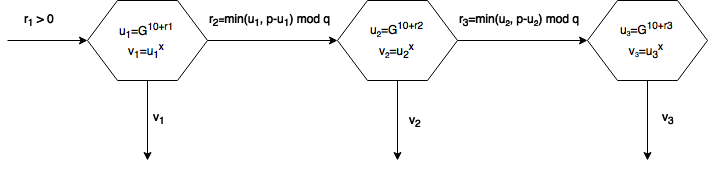
\includegraphics[width=140mm]{prng}
    \caption{Example of a $G_q$-generator.}
    \label{fig:prng}
    \end{figure}
  \end{subproblem}
  \begin{subproblem}
    (5T) NOT SOLVED % We leave this place holder here for improved readability.
  \end{subproblem}
  \begin{subproblem}
    (3T) NOT SOLVED % We leave this place holder here for improved readability.
  \end{subproblem}
  \begin{subproblem}
    (3T) NOT SOLVED % We leave this place holder here for improved readability.
  \end{subproblem}
\end{problem}

\end{document}
